\subfigure[Graph $G$]{
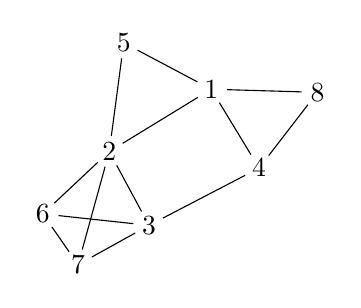
\begin{tikzpicture}[scale = 1.0, every node/.style={circle, inner sep=1pt}]
    \node (v0) at (0.08968749765650905, 0.9699194324453361) {1};
    \node (v1) at (-1.2053866694141455, 0.17836117823866982) {2};
    \node (v2) at (-0.7007765012339914, -0.7589988942400758) {3};
    \node (v3) at (0.697273959143808, -0.031583884618147165) {4};
    \node (v4) at (-1.0217006120092393, 1.5585453027784621) {5};
    \node (v5) at (-2.0488370352520486, -0.6136657725587059) {6};
    \node (v6) at (-1.6013874770008225, -1.2585635251355822) {7};
    \node (v7) at (1.4382648896938393, 0.9300536024094648) {8};
    \foreach \from/\to in {}
        \draw (\from) -- (\to);
    \foreach \from/\to in {}
        \draw[->] (\from) -- (\to);
    \foreach \from/\to in {v1/v0, v3/v0, v4/v0, v7/v0, v2/v1, v4/v1, v5/v1, v6/v1, v3/v2, v5/v2, v6/v2, v7/v3, v6/v5}
        \draw (\from) -- (\to);
    \foreach \from/\to in {}
        \draw[->] (\from) -- (\to);
\end{tikzpicture}}
\subfigure[]{
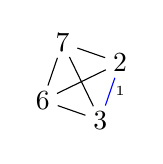
\begin{tikzpicture}[scale = 1.0, every node/.style={circle, inner sep=1pt}]
    \node (v0) at (-0.4508389544742579, -0.24766356929148692) {6};
    \node (v1) at (0.5283327523652851, 0.22871836431842626) {2};
    \node (v2) at (0.27831188359167935, -0.5023284383927149) {3};
    \node (v3) at (-0.20090517631865532, 0.48314395294578205) {7};
\node (v4) at (0.53,-0.135) {\tiny{1}};   
    \foreach \from/\to in {}
        \draw (\from) -- (\to);
    \foreach \from/\to in {}
        \draw[->] (\from) -- (\to);
    \foreach \from/\to in {v1/v0, v2/v0, v3/v0,  v3/v1, v3/v2}
        \draw (\from) -- (\to);
    \foreach \from/\to in {}
        \draw[->] (\from) -- (\to);
\draw[blue] (v1) to (v2);
\end{tikzpicture}}
\subfigure[]{
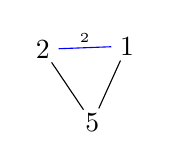
\begin{tikzpicture}[scale = 1.0, every node/.style={circle, inner sep=1pt}]
    \node (v0) at (-0.745936713061192, 0.19701960702269894) {2};
    \node (v1) at (-0.11840649292129297, -0.7353394032199583) {5};
    \node (v2) at (0.32245648565085894, 0.23752940989148924) {1};
\node (v3) at (-0.215,0.34) {\tiny{2}};   
    \foreach \from/\to in {}
        \draw (\from) -- (\to);
    \foreach \from/\to in {}
        \draw[->] (\from) -- (\to);
    \foreach \from/\to in {v1/v0, v2/v1}
        \draw (\from) -- (\to);
    \foreach \from/\to in {}
        \draw[->] (\from) -- (\to);
\draw[blue] (v0) to (v2);
\end{tikzpicture}}
\subfigure[]{
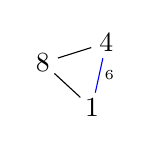
\begin{tikzpicture}[scale = 1.0, every node/.style={circle, inner sep=1pt}]
    \node (v0) at (0.320440056973322, -0.60274184488282) {1};
    \node (v1) at (-0.30275783589298294, -0.027775443839053664) {8};
    \node (v2) at (0.5021089379929771, 0.2252723900354792) {4};
\node (v3) at (0.54,-0.185) {\tiny{6}};    
    \foreach \from/\to in {}
        \draw (\from) -- (\to);
    \foreach \from/\to in {}
        \draw[->] (\from) -- (\to);
    \foreach \from/\to in {v1/v0, v2/v1}
        \draw (\from) -- (\to);
    \foreach \from/\to in {}
        \draw[->] (\from) -- (\to);
\draw[blue] (v0) to (v2);
\end{tikzpicture}}
\subfigure[]{
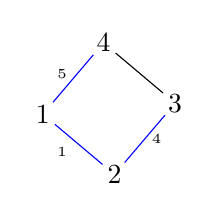
\begin{tikzpicture}[scale = 1.0, every node/.style={circle, inner sep=1pt}]
    \node (v0) at (0.8864325058435051, 0.0756469152993952) {3};
    \node (v1) at (0.11573116481555798, -0.8300942249874552) {2};
    \node (v2) at (-0.7938908246958859, -0.0636352779491744) {1};
    \node (v3) at (-0.023189461604259744, 0.8421058469683372) {4};
\node (v4) at (-0.55,-0.55) {\tiny{1}};
\node (v5) at (-0.55,0.45) {\tiny{5}};
\node (v6) at (0.65,-0.38) {\tiny{4}};    
    \foreach \from/\to in {}
        \draw (\from) -- (\to);
    \foreach \from/\to in {}
        \draw[->] (\from) -- (\to);
    \foreach \from/\to in { v3/v0}
        \draw (\from) -- (\to);
    \foreach \from/\to in {}
        \draw[->] (\from) -- (\to);
\draw[blue] (v2) to (v1);
\draw[blue] (v0) to (v1);
\draw[blue] (v2) to (v3);        
\end{tikzpicture}}
\subfigure[Triple bonds]{
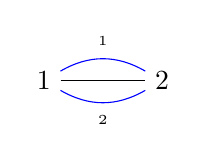
\begin{tikzpicture}
%
% punto inicial, grado inicial, final, radio
\node[] (1) at (0,0) {1};
\node[] (2) at (1.5,0) {2};
\node[] (3) at (0.75,0.5) {\tiny{1}};
\node[] (4) at (0.75,-0.5) {\tiny{2}};
%
%\draw (2,0) node[right]  {$A$};
%\draw (2,0) node  {$A$};
% above, below, right, left,
% above left, above right, below left, below right
\draw (1) to (2);
\draw[blue] (1) to[bend right] (2);
\draw[blue] (2) to[bend right] (1);
%
\end{tikzpicture}
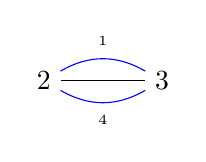
\begin{tikzpicture}
%
% punto inicial, grado inicial, final, radio
\node[] (1) at (0,0) {2};
\node[] (2) at (1.5,0) {3};
\node[] (3) at (0.75,0.5) {\tiny{1}};
\node[] (4) at (0.75,-0.5) {\tiny{4}};
%
%\draw (2,0) node[right]  {$A$};
%\draw (2,0) node  {$A$};
% above, below, right, left,
% above left, above right, below left, below right
\draw (1) to (2);
\draw[blue] (1) to[bend right] (2);
\draw[blue] (2) to[bend right] (1);
%
\end{tikzpicture}
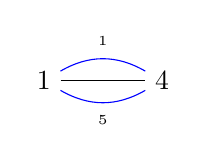
\begin{tikzpicture}
%
% punto inicial, grado inicial, final, radio
\node[] (1) at (0,0) {1};
\node[] (2) at (1.5,0) {4};
\node[] (3) at (0.75,0.5) {\tiny{1}};
\node[] (3) at (0.75,-0.5) {\tiny{5}};
%
%\draw (2,0) node[right]  {$A$};
%\draw (2,0) node  {$A$};
% above, below, right, left,
% above left, above right, below left, below right
\draw (1) to (2);
\draw[blue] (1) to[bend right] (2);
\draw[blue] (2) to[bend right] (1);
%
\end{tikzpicture}}